\documentclass{article}[a4paper,12pt]
\usepackage{pst-knot}
\usepackage{graphicx}
\begin{document}

    \section{Knot $4_1$}

    \begin{itemize}
        \item Generators: $a,b$
        \item Relator: $abbbaBAAB$
        \item Alexander polynomial: $t^2 - 3t + 1$
    \end{itemize}

    \begin{figure}[h]
        \centering
        \begin{pspicture}(-2,-2)(2,2)
            \psKnot[linewidth=3pt,linecolor=blue](0,0){4-1}
        \end{pspicture}
        \caption{Knot $4_1$}
        \label{fig:knot_4_1}
    \end{figure}

    In this section, we consider the knot $4_1$ with generators $a, b$ and the relator $abbbaBAAB$.
    The associated Alexander polynomial is $t^2 - 3t + 1$, and Figure~\ref{fig:knot_4_1} illustrates the geometric representation of this knot.
    We interpret each symbol in the relator $abbbaBAAB$ as an operator:
    $a$ as a multiplicator $\otimes_t$, $b$ as an additor $\oplus_1$, $A$ as a divisor $\oslash_t$, and $B$ as a subtractor $\ominus_1$, where $t$ is an indeterminate variable.
    In the arithmetic expression space $H$, this relator corresponds to a closed loop path, viewed as a threadlike expression.

    \begin{figure}[h]
        \centering
        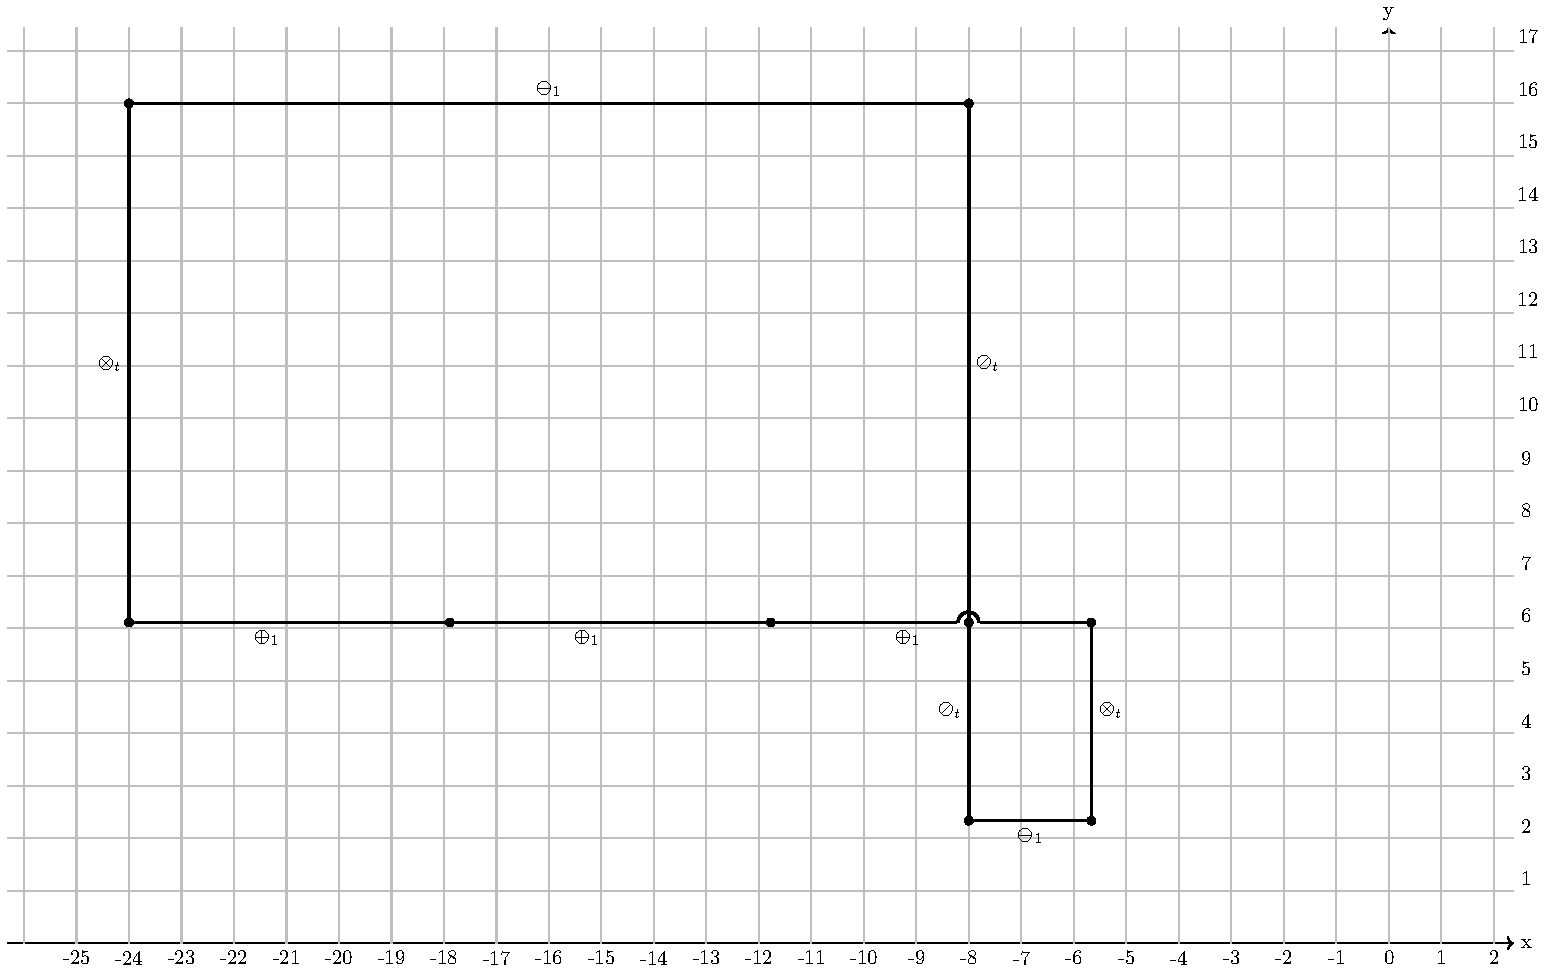
\includegraphics[width=0.8\textwidth]{images/knot_4_1}
        \caption{Relator in the arithmetic expression space $H$}
        \label{fig:relator}
    \end{figure}

    Applying the group action on a real number $x$ from right to left gives:
    \[
        (((x - 1) t^{-1} t^{-1} - 1) t + 1 + 1 + 1) t = x,
    \]
    which forces the Alexander polynomial $t^2 - 3t + 1$ to vanish.
    Solving $t^2 - 3t + 1 = 0$ yields $t = \frac{3 \pm \sqrt{5}}{2}$.
    Equivalently, letting $\phi$ denote the golden ratio, we have $t = \phi^2$ or $t = \phi^{-2}$.

    Although we have shown how applying the relator $abbbaBAAB$ as an arithmetic operation leads to the equation $t^2 - 3t + 1=0$, which is a vanishing Alexander polynomial for the knot $4_1$, the deeper reason behind this connection remains unclear.
    We conjecture that a more geometric interpretation of the Alexander polynomial---and how it encodes the knot's topological features—will illuminate why this algebraic path in $H$ corresponds precisely to the polynomial that characterizes the knot's properties.

\end{document}

